% !TEX encoding = UTF-8 Unicode

\documentclass[BIF,Seminar,english]{twbook}
\usepackage[utf8]{inputenc}
\usepackage[T1]{fontenc}

\usepackage{minted}
\makeatletter
\providecommand\listacroname{}
\@ifclasswith{twbook}{english}
{%
    \renewcommand\listoflistingscaption{List of source codes}
    \renewcommand\listacroname{List of Abbreviations}
}{%
    \renewcommand\listoflistingscaption{Quellcodeverzeichnis}
    \renewcommand\listacroname{Abk�rzungsverzeichnis}
}
\makeatother

\usepackage{blindtext}


\title{Interface segregation principle}
\author{Peter Oettl}
\studentnumber{1910257146}
\supervisor{DI Wolfgang Berger}
\place{Wien}

\begin{document}

\maketitle
\chapter{SOLID principles}

These principles establish practices that lend to developing software with considerations for maintaining and extending as the project grows. Adopting these practices can also contribute to avoiding code smells, refactoring code, and Agile or Adaptive software development. \cite{SOLID}



\section{S - Single Responsiblity Principle}

The single responsibility principle states that a class should have only a single reason to change throughout its lifetime. This principle ensures that a class exists only for a single reason but can have multiple methods to carry out distinct functions.

\section{O - Open Close Principle}


This principle states that objects should be open for extension but closed for modification. The open and close principle ensures our code is easily extensible without editing or rewriting the existing codebase. Designing software applications using this principle ensures extensibility and the reusability of objects.

\section{L - Liskov Substitution Principle}

This principle illustrates that if a section of your code is extending a superclass, then all subclasses of the superclass should be able to replace the superclass in your code. A section of your code does not have to know which class it is as far as it is a superclass subclass. The application of this principle ensures the easy integration of classes.

\section{I - Interface Segregation Principle}

The I  in SOLID stands for interface segregation, and it simply means that larger interfaces should be split into smaller ones. By doing so, we can ensure that implementing classes only need to be concerned about the methods that are of interest to them.

\section{D - Dependency Inversion Principle}

The dependency inversion principle ensures that classes should not depend on solid classes but should only depend on abstraction. By following this approach, it makes the interchanging of modules and classes or services simple. The dependency inversion principle makes changing dependencies easier.



%\begin{listing}[htbp]
%\begin{minted}{go}
%func main() {
%	gamestore := gamestore.NewGame()
%	reader := bufio.NewReader(os.Stdin)
%	for {
%		fmt.Print("-> ")
%		text, _ := reader.ReadString('\n')
%		text = strings.Replace(text, "\n", "", -1)
%
%		if strings.Compare("buy", text) == 0 {
%			gamestore.BuyGame()
%		}
%		if strings.Compare("install", text) == 0 {
%			gamestore.InstallGame()
%		}
%	}
%}
%
%\end{minted}
%\caption{Go Example}
%\end{listing}

\chapter{Interface segregation principle}


\begin{figure}[!htbp]
\centering
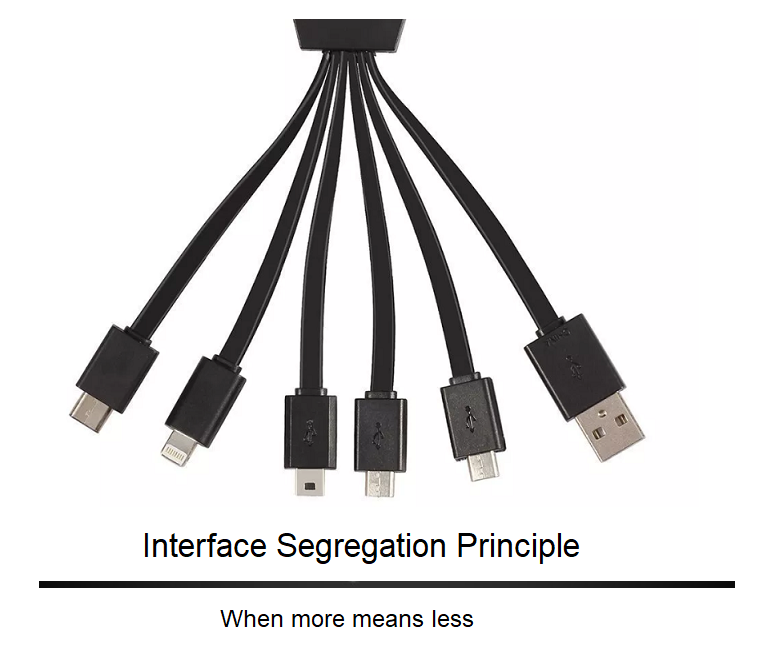
\includegraphics[width=0.5\linewidth]{PICs/ISP}
\caption{Interface segregation principle}\label{Abb1}
\end{figure}



\begin{center} 
 ``Clients should not be forced to depend upon interfaces that they do not use.''\newline
\end{center} 

Im Prinzip kann man das ISP so zusammenfassen: Verwende immer nur die kleinstm�gliche Schnittstelle zu deinen Abh�ngigkeiten. Je mehr Funktionen eine Komponente an ihren Abh�ngigkeiten aufrufen kann, desto abh�ngiger wird sie von ihr. Wenn sich diese Funktionen n�mlich �ndern (z.B. die Signatur einer Methode), muss die nutzende Komponente neu kompiliert werden. Au�erdem k�nnen Funktionen aufgerufen werden, die die nutzende Komponente weder ben�tigt, noch anwenden soll, z.B. die clear()-Methode einer Liste, die sie eigentlich nur durchlaufen soll. Zuletzt m�ssen auch implementierende Klassen von zu gro�en Interfaces f�r sie unn�tige Methoden implementieren, nur um der Schnittstelle zu entsprechen.



\chapter{Practical Example}



\begin{listing}[htbp]
\begin{minted}{java}
interface Bird {
  fly(): void;
  walk(): void;
}

class Duck extends Bird{
    fly(){
        // Duck can fly
    }   
    walk(){
        // Duck can walk
    }
}

class Ostrich extends Bird{
    fly(){
        // Ostrich cant fly... throw some error
    }   
    walk(){
        // Ostrich can walk
    }
}

\end{minted}
\caption{initial scenario}
\end{listing}


\begin{listing}[htbp]
\begin{minted}{java}
interface BirdFly{
    fly(): void;
}

interface BirdWalk{
    walk(): void;
}

class Duck extends BirdFly, BirdWalk{
    fly(){
        // Duck can fly
    }   
    walk(){
        // Duck can walk
    }
}

class Ostrich extends BirdWalk{
    walk(){
        // Ostrich can walk
    }
} 

\end{minted}
\caption{ISP}
\end{listing}



% Hier beginnen die Verzeichnisse.
\clearpage
\bibliographystyle{IEEEtran}
\bibliography{Literatur}
\clearpage

\listoffigures
\clearpage

\phantomsection
\addcontentsline{toc}{chapter}{\listacroname}
\chapter*{\listacroname}
\begin{acronym}[XXXXX]
	\acro{aaa}[aaa]{allaboutapps}
\end{acronym}

%Fix for fhtw_cover

\includegraphics[width=0\linewidth]{PICs/fhtw_cover}

\end{document}
